
% License:
% CC BY-NC-SA 3.0 (http://creativecommons.org/licenses/by-nc-sa/3.0/)
%
%%%%%%%%%%%%%%%%%%%%%%%%%%%%%%%%%%%%%%%%%

%----------------------------------------------------------------------------------------
%	PACKAGES AND OTHER DOCUMENT CONFIGURATIONS
%----------------------------------------------------------------------------------------

\documentclass[paper=a4, fontsize=11pt]{scrartcl} % A4 paper and 11pt font size

\usepackage[T1]{fontenc} % Use 8-bit encoding that has 256 glyphs
\usepackage{fourier} % Use the Adobe Utopia font for the document - comment this line to return to the LaTeX default
\usepackage[english]{babel} % English language/hyphenation
\usepackage{amsmath,amsfonts,amsthm} % Math packages
\usepackage{lipsum} % Used for inserting dummy 'Lorem ipsum' text into the template

\usepackage{caption}
\usepackage{subcaption}
\usepackage{graphicx}

\usepackage{float}

\usepackage{blindtext} %for enumarations

\usepackage[]{hyperref}  %link collor

\usepackage{xargs}                      % Use more than one optional parameter in a new commands
\usepackage[pdftex,dvipsnames]{xcolor}  % Coloured text etc.
% 
\usepackage[colorinlistoftodos,prependcaption,textsize=tiny]{todonotes}
\newcommandx{\unsure}[2][1=]{\todo[linecolor=red,backgroundcolor=red!25,bordercolor=red,#1]{#2}}
\newcommandx{\change}[2][1=]{\todo[linecolor=blue,backgroundcolor=blue!25,bordercolor=blue,#1]{#2}}
\newcommandx{\info}[2][1=]{\todo[linecolor=OliveGreen,backgroundcolor=OliveGreen!25,bordercolor=OliveGreen,#1]{#2}}
\newcommandx{\improvement}[2][1=]{\todo[linecolor=Plum,backgroundcolor=Plum!25,bordercolor=Plum,#1]{#2}}
\newcommandx{\thiswillnotshow}[2][1=]{\todo[disable,#1]{#2}}


%talbe layout to the right
%\usepackage[labelfont=bf]{caption}
%\captionsetup[table]{labelsep=space,justification=raggedright,singlelinecheck=off}
%\captionsetup[figure]{labelsep=quad}

\usepackage{sectsty} % Allows customizing section commands
\allsectionsfont{\centering \normalfont\scshape} % Make all sections centered, the default font and small caps

\usepackage{fancyhdr} % Custom headers and footers
\usepackage{register} % Custom headers and footers
\pagestyle{fancyplain} % Makes all pages in the document conform to the custom headers and footers
\fancyhead{} % No page header - if you want one, create it in the same way as the footers below
\fancyfoot[L]{} % Empty left footer
\fancyfoot[C]{} % Empty center footer
\fancyfoot[R]{\thepage} % Page numbering for right footer
\renewcommand{\headrulewidth}{0pt} % Remove header underlines
\renewcommand{\footrulewidth}{0pt} % Remove footer underlines
\setlength{\headheight}{13.6pt} % Customize the height of the header

\numberwithin{equation}{section} % Number equations within sections (i.e. 1.1, 1.2, 2.1, 2.2 instead of 1, 2, 3, 4)
\numberwithin{figure}{section} % Number figures within sections (i.e. 1.1, 1.2, 2.1, 2.2 instead of 1, 2, 3, 4)
\numberwithin{table}{section} % Number tables within sections (i.e. 1.1, 1.2, 2.1, 2.2 instead of 1, 2, 3, 4)


\setlength\parindent{0pt} % Removes all indentation from paragraphs - comment this line for an assignment with lots of text

\setlength\parskip{10pt}

%----------------------------------------------------------------------------------------
%	TITLE SECTION
%----------------------------------------------------------------------------------------

\newcommand{\horrule}[1]{\rule{\linewidth}{#1}} % Create horizontal rule command with 1 argument of height

\title{	
\normalfont \normalsize 
\horrule{0.5pt} \\[0.4cm] % Thin top horizontal rule
\huge  SafeDE User's Manual\\ % The assignment title
\horrule{2pt} \\[0.5cm] % Thick bottom horizontal rule
}

\author{Francisco Bas} % Your name

\date{\today} % Today's date or a custom date

\usepackage{listings}
\lstdefinelanguage{VHDL}{
	morekeywords={
		library,use,all,entity,is,port,in,out,end,architecture,of,
		begin,and
	},
	morecomment=[l]--
}

\usepackage{xcolor}
\colorlet{keyword}{blue!100!black!80}
\colorlet{comment}{green!90!black!90}
\lstdefinestyle{vhdl}{
	language     = VHDL,
	basicstyle   = \ttfamily,
	keywordstyle = \color{keyword}\bfseries,
	commentstyle = \color{comment},
	framexleftmargin = 15pt
}

\usepackage{caption}
\DeclareCaptionFont{white}{\color{white}}
\DeclareCaptionFormat{listing}{%
	\parbox{\textwidth}{\colorbox{gray}{\parbox{\textwidth}{#1#2#3}}\vskip-4pt}}
\captionsetup[lstlisting]{format=listing,labelfont=white,textfont=white}
\lstset{frame=lrb,xleftmargin=\fboxsep,xrightmargin=-\fboxsep}


\begin{document}
%\nocite{*}
\maketitle % Print the title

\newpage
\tableofcontents

%----------------------------------------------------------------------------------------
%	Section 1
%----------------------------------------------------------------------------------------

\newpage
\section{Overview}
\label{chapter1}

\subsection{SafeDM description}
\label{descrption_subsec}

SafeDM is a hardware Diversity Monitor that quantifies the diversity between two redundant processors to guarantee that CCF will not go unnoticed, and without needing to deploy lockstepped cores. SafeDM takes advantage of the fact that diversity naturally exists due to the complexity of the system to develop the safety concept. Each cycle SafeDM computes one signature per core summarizing their internal state. Both signatures are compared and if they coincide, lack of diversity is reported.

SafeDM is instantiated in the SoC as an APB slave\footnote{Based on AMBA 2.0 specification}. SafeDM raises an output each cycle that diversity is missed between cores. SafeDM also has an internal counter that is increased by one each cycle that there is lack of diversity. The value of this counter can be retrieved through the APB bus reading the appropriate register. SafeDM only reports a lack of diversity in the system and it is up to the user to determine the proper actions in the event of missing diversity.


\begin{figure}[H]
	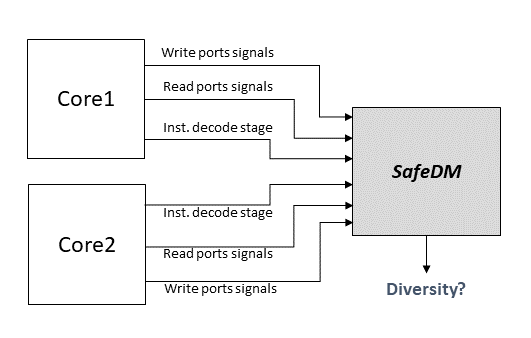
\includegraphics[keepaspectratio,width=\columnwidth]{img/SafeDM_scheme.png}
        \caption{SafeDM simplified scheme.} 
	\label{fig:simplified_scheme}
\end{figure}

Figure \ref{fig:simplified_scheme} shows a simplified scheme of SafeDM connected to two redundant processors. Internally, SafeDM generates two different signatures that later are concatenated into a single one: instruction and data signatures. Some internal signals from the pipeline and the register file are required to calculate those signatures.

The signatures are generated by storing the last instructions processed in the decode stage (Figure \ref{fig:instruction_signature}) and the last values read from the register file ports in FIFOs (Figure \ref{fig:register_signature}). 


\begin{figure}[H]
	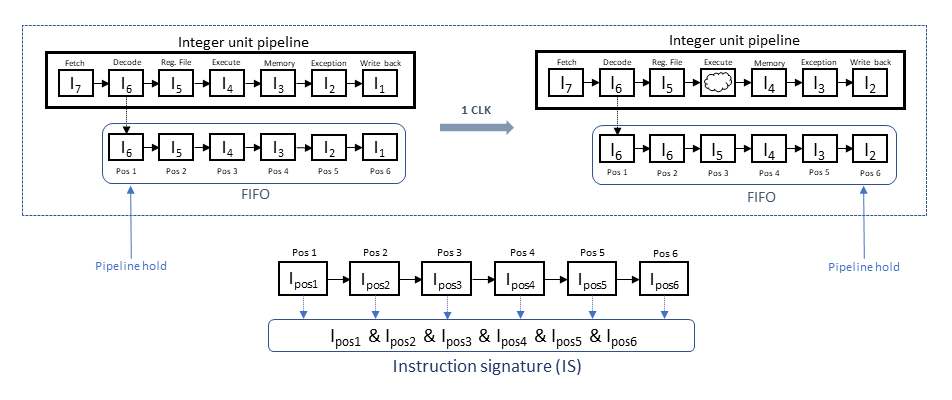
\includegraphics[keepaspectratio,width=\columnwidth]{img/SafeDM_instructions.png}
        \caption{Instructions signature scheme.} 
	\label{fig:instruction_signature}
\end{figure}

\begin{figure}[H]
	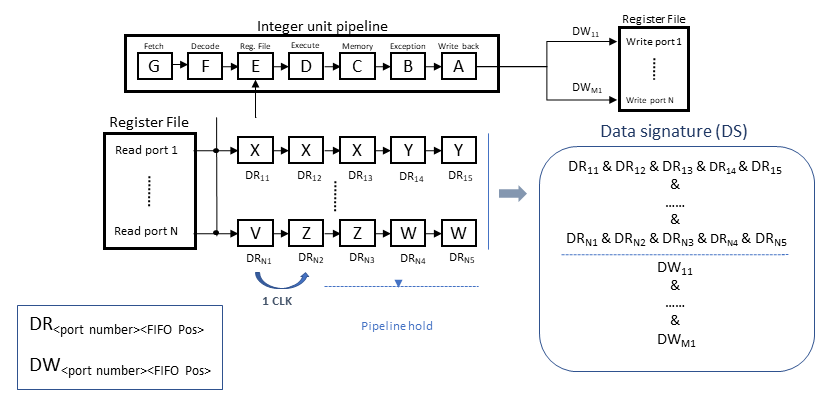
\includegraphics[keepaspectratio,width=\columnwidth]{img/SafeDM_registers.png}
        \caption{Registers signature scheme.}
	\label{fig:register_signature}
\end{figure}

SafeDM offers some advantages in comparison to lockstep approaches:
\begin{itemize}
	\item \textbf{Performance:} Classical tight-lockstep approach employs two cores that are seen as one by the user, thus halving the performance. A pair of redundant cores monitored by SafeDM can execute different tasks at any time.
	\item \textbf{Instructions stream:} Other lockstep approaches as light\-lockstep avoid the performance penalty of the tight\-lockstep but require identical instructions streams. This prevents this solution from executing parallel applications or handling the system's inputs and outputs. SafeDM overcomes this limitation.
    \item \textbf{Low intrusiveness:} SafeDM can be implemented in a SoC performing only a few modifications in the design. SafeDM only needs a few signals to calculate the signatures.
\end{itemize}



\subsection{Licensing}

This BSC IP core module is freely provided under the terms of the MIT License.



\hspace{5cm}


%----------------------------------------------------------------------------------------
%	Section 2
%----------------------------------------------------------------------------------------

\section{Product specification}



\subsection{Configuration options}
\label{confg_chap}

Several SafeDM parameters have to be correctly configured for SafeDM to adapt to the concrete architecture of the replicated cores. Table \ref{generics} shows SafeDM VHDL generics that allow configuring the hardware design.

Table \ref{generics} shows SafeDM configuration parameters (VDHL generics). 
\\
\begin{table}[H]
	\caption{Configuration options (VHDL ports)}
	\label{generics}
	\centering
	\begin{small}
		\begin{tabular}{|l|p{6cm}|l|l|}
			\hline
			\textbf{Generic} & \textbf{Description}  & \textbf{Allowed range}  & \textbf{Default}\\
			\hline
			CODING\_METHOD   & When it is set to 1, ECC (Error Correction Codes) redundant bits are generated for the instructions and register value inputs. SafeDM stores the ECC\-generated bits instead of storing all  instruction and register bits saving FPGA resources.  All the original input bits are stored if this generic is set to 0. & 0 to 1 & 0\\
			\hline
			CODING\_BITS\_REG  & Register FIFO width in bits. It depends on the selected coding method and the size of the registers of the cores. & - & 64\\
			\hline
			CODING\_BITS\_INST & Instruction FIFO width in bits. It depends on the selected coding method and the size of the instructions of the cores. & - & 32\\
			\hline
			REGS\_FIFO\_POS    & Register FIFO number of positions. & - & 5\\
			\hline
			INST\_FIFO\_POS    & Instruction FIFO number of positions. & - & 6\\
			\hline
		\end{tabular}
	\end{small}
\end{table}

%use any kind of rerence to link the parameters of the table with the explanations?¿?¿
%Why is this error appearing?

When the CODING\_METHOD generic is set to 1, ECC are calculated applying the extended hamming code method. For inputs that are a power of 2, the output is \(output\_bits=log2(input\_bits)+2\). For instance, if the instruction length of the cores is 32, the output length after applying the extended hamming code method will have \(5+2=7\) bits. Therefore, CODING\_BITS\_INST generic must be set to 7. 

As explained before in section \ref{descrption_subsec}, SafeDM generates two signatures storing the last instructions from the decode stage, and the last values read and written in the register file. To generate the signatures, it employs two FIFOs, one for each signature. The Instruction FIFO depth is configured using the INST\_FIFO\_POS generic. Its value must be equal to the number of pipeline stages from decode to the end of the pipeline including decode. The register FIFO depth is configured using the REGS\_FIFO\_POS generic. Its value must be equal to the number of pipeline stages from the register file stage to the end of the pipeline including the register file stage.

Different core architectures can have a different number of read and write ports in the register file or they can be single or multiple\-issue with a different number of lanes. This parameters can be configured in the file containing the type definitions \textit{diversity\_types\_pkg.vhd} changing the value of the constants \textit{lanes\_number} and \textit{read\_ports}. Notice that SafeDM is not devised to work with out\-of\-order superscalar processors. 


\subsection{Port Descriptions}
\label{port_description}

Table \ref{t_ports} shows the interface of the IP core (VHDL ports).
\begin{table}[H]
	\caption{Signal descriptions (VHDL ports)}
	\label{t_ports}
	\centering
	\begin{footnotesize}
	\begin{tabular}{|l|l|c|p{6cm}|l|}
		\hline
		\textbf{Signal name} & \textbf{Type} & \textbf{I/O} & \textbf{Description} & \textbf{Active}\\
		\hline
		RSTN                 & STD\_LOGIC                & I & Reset                           & Low\\
		\hline
		CLK                  & STD\_LOGIC                & I & AHB master bus clock            & -\\
		\hline
		APBI\_PSEL\_I        & STD\_LOGIC                & I & APB slave selection signal      & -\\
		\hline
		APBI\_PADDR\_I       & STD\_LOGIC\_VECTOR        & I & APB address signal              & -\\
		\hline
		APBI\_PENABLE\_I     & STD\_LOGIC                & I & APB enable signal               & -\\
		\hline
		APBI\_PWRITE\_I      & STD\_LOGIC                & I & APB read/write selection signal & -\\
		\hline
		APBI\_PWDATA\_I      & STD\_LOGIC\_VECTOR        & I & APB write data signal           & -\\
		\hline
		APBI\_PRDATA\_O      & STD\_LOGIC\_VECTOR        & O & APB read data signal            & -\\
		\hline
		INSTRUCTIONS\_I      & INSTRUCTION\_TYPE\_VECTOR & I & This type definition is a two-vector positions (one for each core) of the type \textit{instruction\_type}. This type includes an instruction value and a bit indicating if that instruction is valid per lane. The instructions value signals should come from the decode stage. & -\\
		\hline
		REGISTERS\_I         & REGISTER\_TYPE\_VECTOR    & I & This type definition is a two-vector positions (one for each core) of the type \textit{register\_type}.This type definition includes a register value and a bit indicating if that register is read per register file read port. The registers value should come from the register file. & -\\
		\hline
		HOLD\_I              & STD\_LOGIC\_VECTOR        & I & This signal is a two-bits vector containing the hold signal of each core. The hold signal is set to 1 when the core pipeline is held.  & High\\
		\hline
		DIVERSISTY\_LACK\_O  & STD\_LOGIC                & O & This signal rises when the signatures from both cores coincide meaning that there is no diversity between both core replicas. & High\\
		\hline
	\end{tabular}
\end{footnotesize}
\end{table}

As explained later in section \ref{implementation}, SafeDM top VHDL file should be instantiated in an APB wrapper to drive the APB signals to SafeDM top. This wrapper should also define the input signals of the types \textit{instruction\_type\_vector} and \textit{register\_type\_vector} and wire those signals with the ones coming from the cores. This kind of design allows configuring the number of lanes and read ports without modifying the architecture ports.


\subsection{Register space}

SafeDM has only two registers that can be accessed through normal store and load operations.  

The first register is used to reset SafeDM and start SafeDM operation:

\begin{register}{H}{SafeDM configuration register}{0x00}
	\label{cfg0}
	\regfield{Reserved}{30}{2}{{0}}
	\regfield{Enable}{1}{1}{{0}}
	\regfield{Soft\_reset}{1}{0}{{0}}
	\reglabel{Reset value}\regnewline
\end{register}

Once the enable bit is set to 1, SafeDM will start monitoring the diversity.

The second register contains the number of cycles in which SafeDM detected lack of diversity.

\begin{register}{H}{No-diversity cycles counter}{0x04}
	\label{no_div_cycles_reg}
	\regfield{No-diversity cycles}{32}{0}{{0}}
	\reglabel{Reset value}\regnewline
\end{register}

To reset the count SafeDM has to be reset.


\subsection{Resources}



\hspace{2cm}




\section{Clocking and reset}

\subsection{Clocking}
SafeDM has a single input clock. You should connect the appropriate AHB bus clock to this clock input. 

\subsection{Resets}
SafeDM reset \textit{rstn} is an active-Low synchronous reset to the core. All registers are reset to power-on conditions. Apart from the external reset signal, SafeDM can be reset through the configuration APB register \ref{cfg0}.  




%\newpage
\section{Implementing the IP core}
\label{implementation}

As mention in the section \ref{port_description}, to implement SafeDM we need a wrapper. The function of this wrapper is to adapt the input signals. Below is an example of a wrapper used in a SoC designed by Cobham Gaisler. The SoC cores are Noel-V 64-bits cores. The noel-V core is dual-issue and has four read register file ports.

As you can see in the example, the APB signals are a custom type defined by gaisler that has to be converted into \textit{std\_logic} and \textit{std\_logic\_vector} types. On the other hand the \textit{std\_logic} and \textit{std\_logic\_vector} types of the instructions and registers inputs have to be converted into the \textit{instruction\_type\_vector} and \textit{register\_type\_vector\ types}.


%Try to put it more clean and beatuful
\belowcaptionskip=-10pt
\begin{lstlisting}[label=ins-prot,caption=SafeDM instance example,style=vhdl,frame=none,tabsize=2]

library ieee; 
use ieee.std_logic_1164.all;
use ieee.numeric_std.all;
use ieee.math_real.all;
-- AMBA 2.0 Cobham Gaisler's library 
-- It defines AHB and APB specific types
library grlib;
use grlib.amba.all;
use grlib.devices.all;
-- Library containing SafeDM
library bsc;
use bsc.diversity_types_pkg.all;
use bsc.diversity_components_pkg.SafeDM_top;


entity apb_wrapper_diversity is
	generic (
		-- APB generics
		pindex : integer := 0;
		paddr  : integer := 0;
		pmask  : integer := 16#fff#;
		-- SafeDM configuration
		coding_method    : integer := 1;
		coding_bits_reg  : integer := 64;
		coding_bits_inst : integer := 32;
		regs_fifo_pos    : integer := 5;
		inst_fifo_pos    : integer := 6
	);
	port (
		rstn   : in std_logic;
		clk    : in std_logic;
		-- Apb signals
		apbi_i : in apb_slv_in_type;
		apbo_o : out apb_slv_out_type;
		-- Instructions sign signals (both cores)
		-- Core 1
		lane1_inst_value_1_i : in std_logic_vector(31 downto 0); 
		lane2_inst_value_1_i : in std_logic_vector(31 downto 0);  
		inst_valid_1_i   : in std_logic_vector(1 downto 0); 
		-- Core 2
		lane1_inst_value_2_i : in std_logic_vector(31 downto 0);  
		lane2_inst_value_2_i : in std_logic_vector(31 downto 0);  
		inst_valid_2_i   : in std_logic_vector(1 downto 0); 
		-- Registers sign signals (both cores)
		-- Core 1
		port1_ren_1_i   : in std_logic;
		port2_ren_1_i   : in std_logic;
		port3_ren_1_i   : in std_logic; 
		port4_ren_1_i   : in std_logic; 
		port1_rdata_1_i : in std_logic_vector(63 downto 0);   
		port2_rdata_1_i : in std_logic_vector(63 downto 0);
		port3_rdata_1_i : in std_logic_vector(63 downto 0);
		port4_rdata_1_i : in std_logic_vector(63 downto 0);
		-- Core 2
		port1_ren_2_i   : in std_logic;
		port2_ren_2_i   : in std_logic;
		port3_ren_2_i   : in std_logic; 
		port4_ren_2_i   : in std_logic; 
		port1_rdata_2_i : in std_logic_vector(63 downto 0);   
		port2_rdata_2_i : in std_logic_vector(63 downto 0);
		port3_rdata_2_i : in std_logic_vector(63 downto 0);
		port4_rdata_2_i : in std_logic_vector(63 downto 0);
		-- Hold signals
		hold_1_i : in std_logic;
		hold_2_i : in std_logic;
		-- Lack of diversity
		diversity_lack_o : out std_logic
	);
	end;

architecture structural of apb_wrapper_diversity is
	

	-- APB configuration ----------------------------------------
	constant REVISION  : integer := 0;
	constant VENDOR_ID : integer := 16#0e#;
	constant DEVICE_ID : integer := 16#002#;

	constant PCONFIG : apb_config_type := (
	0 => ahb_device_reg (VENDOR_ID, DEVICE_ID, 0, REVISION, 0),
	1 => apb_iobar(paddr, pmask));
	-------------------------------------------------------------

	
	-- Inputs to SafeDM
	signal instructions : instruction_type_vector;
	signal registers    : register_type_vector;
	signal hold : std_logic_vector(1 downto 0);

begin

	-- SafeDM inputs are driven to the input register_type_vector and 
	-- instruction_type_vector types.
	-- INSTRUCTIONS
	-- Core 1 assignation
	instructions(0).inst_value(0) <= lane1_inst_value_1_i;
	instructions(0).inst_value(1) <= lane2_inst_value_1_i;
	instructions(0).valid     <= inst_valid_1_i;  
	-- Core 2 assignation
	instructions(1).inst_value(0) <= lane1_inst_value_2_i;
	instructions(1).inst_value(1) <= lane2_inst_value_2_i;
	instructions(1).valid     <= inst_valid_2_i;  
	-- REGISTERS
	-- Core 1 assignement
	registers(0).value(0) <= port1_rdata_1_i; 
	registers(0).value(1) <= port2_rdata_1_i; 
	registers(0).value(2) <= port3_rdata_1_i; 
	registers(0).value(3) <= port4_rdata_1_i; 
	registers(0).ren(0)   <= port1_ren_1_i; 
	registers(0).ren(1)   <= port2_ren_1_i; 
	registers(0).ren(2)   <= port3_ren_1_i; 
	registers(0).ren(3)   <= port4_ren_1_i; 
	-- Core 2 assignement
	registers(1).value(0) <= port1_rdata_2_i; 
	registers(1).value(1) <= port2_rdata_2_i; 
	registers(1).value(2) <= port3_rdata_2_i; 
	registers(1).value(3) <= port4_rdata_2_i; 
	registers(1).ren(0)   <= port1_ren_2_i; 
	registers(1).ren(1)   <= port2_ren_2_i; 
	registers(1).ren(2)   <= port3_ren_2_i; 
	registers(1).ren(3)   <= port4_ren_2_i; 
	-- Hold signals
	hold <= hold_2_i & hold_1_i;

	
	apb_diversity_inst : SafeDM_top
	generic map(
		coding_method    => coding_method,
		coding_bits_reg  => coding_bits_reg,
		coding_bits_inst => coding_bits_inst,
		regs_fifo_pos    => regs_fifo_pos,
		inst_fifo_pos    => inst_fifo_pos
		)
	port map(
		rstn          => rstn, 
		clk           => clk, 
		-- Apb signals: From Cobham Gailer's types
		-- to std_logic and std_logic_vectors
		apbi_psel_i     => apbi_i.psel(pindex),     
		apbi_paddr_i    => apbi_i.paddr,    
		apbi_penable_i  => apbi_i.penable,  
		apbi_pwrite_i   => apbi_i.pwrite,   
		apbi_pwdata_i   => apbi_i.pwdata,   
		apbo_prdata_o   => apbo_o.prdata,   
		-- Singals to calculate sigantures
		-- Instructions signature inputs
		instructions_i => instructions,
		-- Registers signatures inputs
		registers_i => registers,
		-- Hold signals
		hold => hold,
		-- Lack of diversity flag
		diversity_lack_o => diversity_lack_o
		);


	-- APB bus output signals
	apbo_o.pirq    <= (others => '0');
	apbo_o.pindex  <= pindex;
	apbo_o.pconfig <= PCONFIG;
	
end;  

\end{lstlisting}


\hspace{2cm}


\section{Library dependences}
Table \ref{dep_tab} shows the VHDL libraries used when instantiating SafeDM.

\begin{table}[H]
	\caption{Library dependencies}
	\label{dep_tab}
	\centering
	\begin{small}
	\begin{tabular}{|l|l|l|p{6cm}|}
		\hline
		\textbf{Library} & \textbf{Package}  & \textbf{Imported units}  & \textbf{Description} \\
		\hline
		IEEE & std\_logic\_1164 & Types & Standard logic types\\
		\hline
		IEEE & numeric\_std & Functions and types & Arithmetic functions and signed and unsigned types\\
		\hline
		IEEE & math\_real & Constants and functions & Mathematical functions and constants\\
		\hline
		BSC & diversity\_types\_pkg & Types and constants & Custom SafeDM types and configuration constants\\
		\hline
		BSC & diversity\_components\_pkg & SafeDM components & SafeDM component definitions\\
		\hline
	\end{tabular}
\end{small}
\end{table}


\hspace{2cm}


\section{Simulation}

\subsection{Test Bench}

The design also contains a test bench. First, the test bench resets and enables SafeDM writing in the configuration register through the APB interface. The instructions and registers values fed as inputs to SafeDM are randomly generated using pseudo-random number generators. At some point, generated instructions and registers values of both cores coincide, simulating a lack of diversity scenario. Later, the counter storing the cycles where the system lacked diversity is read and compared with the expected value. The test bench will fail if the expected and obtained values do not coincide.

Changing the constants \textit{lanes\_number} and \textit{read\_ports} in the VHDL package \textit{diversity\_type\_pkg.vhd} will also modify the test bench to generate the proper inputs for the SafeDM module.



\subsection{Performing simulation}

We have performed the simulation using \textit{Questa Sim 10.7c}. You can reproduce the simulation using the Makefile inside the folder \textit{tb}. Several recipes:

\begin{itemize}
    \item \textbf{compile:} It creates the work and safety libraries and compiles all the VHDL files.
    \item \textbf{vsim-launch:} It compiles and launches the QuestaSim graphical user interface simulation.
    \item \textbf{vsim:} It compiles and runs the simulation in batch mode.
    \item \textbf{launch-tb:} It compiles, runs the simulation in batch mode and analyzes the test-bench results.
    \item \textbf{clean:} It removes temporal files.                                                         
\end{itemize}

\end{document}



\input{7-Section.tex}





\end{document}
